% Define the scope, extend, and how of the study
\chapter{Methodology}
\label{sec:methodology}
% \begin{figure}
%   \centering
%   \graphicspath{ {../schemas/methodology/} }
%   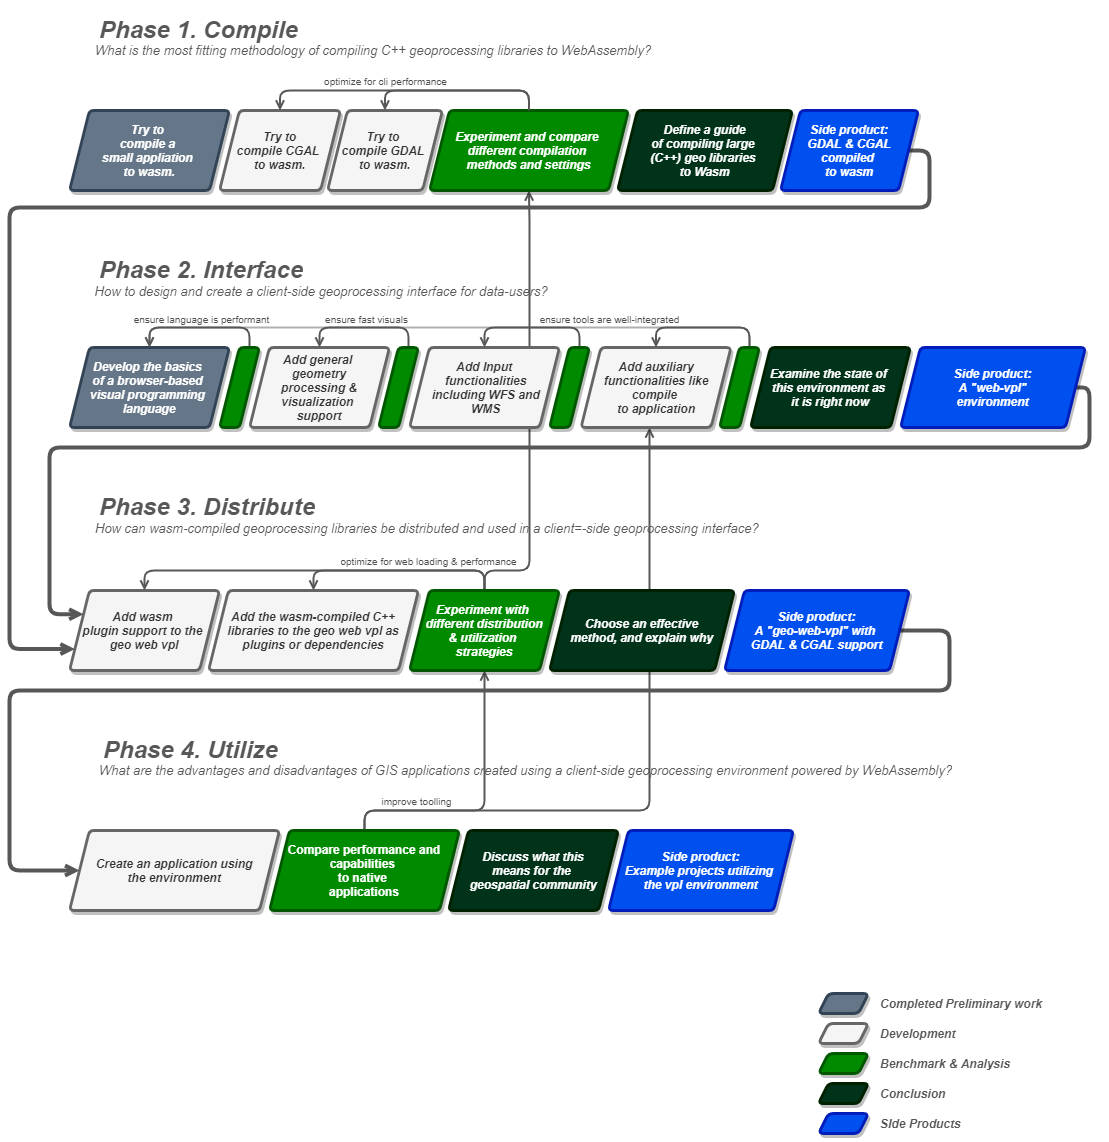
\includegraphics[width=14cm]{method.png}
%   \caption{Methodology schema}
%   \label{fig:method}
% \end{figure}

% The methodology used can be characterized as both incremental and iterative. Its incremental nature means that every phase, and every step within a phase, will produce meaningful in-between products \& results. This ensures the study will be insightful, even in the case the full scope of this study might become unfeasible. It is also vital for making the methodology iterative. 

% The study's iterative nature means that analysis and benchmarks will not be postponed until the end of the study, and will instead be an intricate part of each step. This makes sure obstacles are discovered early, and the trajectory of the study can be adjusted dynamically.  

% Every phase contains a number of development \& analysis steps. The reasoning behind these steps are covered by the following sub-chapters.  




%%%%%%%%%%%%%%%%%%%%%%%%%%%%%%%%%%%%%%%%%%%%%%%%%%%%%%%%%%%%%%%%%%%%%%%%%%%%%%%

\subsection{Phase 1: Compile}

% not as easy 
% The study starts out with the assumption that WebAssembly must be utilized to properly compile and run existing geoprocessing libraries in a browser. This might not be as easy as using normal compilers, based on the experience gained by preliminary work (See \autoref{sec:preliminary-wasm}). WebAssembly is containerized and makes no assumptions about its source language \cite{haas_bringing_2017}, making aspects such as an SDK, sub-dependencies called using environment variables, and IO (file reading and writing) possible obstacles. These aspects might be solved by using or writing wrapper libraries and using file system workarounds, as proposed by \cite{jangda_not_2019}. 

% question & steps to answer
The first sub-question is dedicated to overcoming Obstacle 1, and uses the related works on \ac{wasm}. It goes: \textbf{"What is the most fitting methodology of compiling C++ geoprocessing libraries to WebAssembly?"}.
We specify ourselves to C++, since this seems to be the language of choice for almost all well established geoprocessing libraries. 
'Fitting' in this context refers to the specific requirements posed by geoprocessing libraries. 
The libraries are large and complex, and the geodata used as input even more so. 
This means special attention will be given to these aspects. 
Standard compiler effectiveness criteria, such as portability (smallest file size), and performance, will also be considerations during the assessment of methodologies.  

While the question poses to find the \textit{best} compilation method, if it turns out that only one method makes it possible to compile sizable geo-libraries, this phase will nonetheless regard itself as successful. The question will have to be rephrased in that case. 

% performance
\subsubsection*{Performance}
The performance benefit of WebAssembly is an important component of why WebAssembly might be beneficial for client-side geoprocessing. As such, this phase is interested in confirming whether this is the case for geoprocessing applications. Once a sufficient compilation method is found, individual functions of geoprocessing libraries will be benchmarked using three different methods: 

\begin{itemize}
  \item Compiled and run as native binary (g++), 
  \item Compiled to wasm, run natively (WASI),
  \item Compiled to asm.js, run natively (NODE.js),
\end{itemize}

% why cgal & GDAL
\subsubsection*{Test Cases}
CGAL \& GDAL will be used as examples of "C++ geoprocessing libraries" for this phase. For one, these libraries are well established and relevant to geoprocessing as a whole. Many other geo-libraries depend on them. Moreover, they are large and complex, making it highly likely the problems described by related works will be encountered. We could choose more simple libraries, but this will not be representative of most C++ geoprocessing libraries. 

While CGAL \& GDAL will be this phase's primary subject, the answer of this sub-question aims to be applicable to all geoprocessing libraries. 

%%%%%%%%%%%%%%%%%%%%%%%%%%%%%%%%%%%%%%%%%%%%%%%%%%%%%%%%%%%%%%%%%%%%%%%%%%%%%%%
\newpage
\subsection{Phase 2: Interface}

Phase 2 is dedicated to overcoming Obstacle 2, assisted by the related works on the geoweb. Phase 2 seeks to not only make geoprocessing runnable, but actually usable, and usable to a wide audience of "data-users". This quest is posed using the research question: \textbf{How to design and create a client-side geoprocessing environment for data-users?}. 

Phase 2 will primarily be about implementing the foundations of the use-case application 'GeoFront'. None of the existing web-based \ac{vpl}'s were deemed acceptable for the scope of this study, so the application will have to be created from scratch. 
The application will be created using JavaScript, or its type-save equivalent TypeScript. 
A choice can be made to write the whole environment as a native application which then, as a whole, can be published to the web using WebAssembly. 
This would probably be the most performant. 
However, referring back to the FAIR principles of \cite{mark_d_wilkinson_fair_2016}, this would be detrimental to the concept of Interoperability and Reusability. 
We wish the environment to contain small, standalone components which could be useful in and of themselves. 
For example, users might want to integrate a geodata process on their own website without the full \ac{gui} attached.

The modern web contains many technologies we can possibly use to facilitate all required features. WebGL offers the ability to efficiently visualize 3D data. The 2d canvas API and SVG's can be used to visualize 2D data. HTML can be used to build the interface.

\subsubsection*{Steps}

Just like the entire study, the development trajectory during phase 2 will be done incrementally, ensuring results can be shown during all steps of the development. 
The first step of the phase will consist of creating the basics of the \ac{gui} itself. a basic \ac{vpl} will be created which can only process boolean statements. The second step adds types, geometry, and the visualization of this geometry in 3D, as well as textures / images in 2d. The third step will add geospatial data support, like Web Feature Services, Web Map Services, and coordinate reference systems.  

%%%%%%%%%%%%%%%%%%%%%%%%%%%%%%%%%%%%%%%%%%%%%%%%%%%%%%%%%%%%%%%%%%%%%%%%%%%%%%%

\subsection{Phase 3: Distribute}

% performant and sharable geoprocessing
% portability


The third phase is characterized by harmonizing the results of Phase 1 and 2. 
The related works pointed out that WebAssembly can only truly be tested within a realistic use-case scenario, So this Phase intends to do just that.
The research question goes: \textbf{What is the best way of distributing wasm-compiled geoprocessing libraries, in order to use them within a client-side geoprocessing environment?}. 
This phase can be seen as a continuation of phase 1, but where the compilation research of phase 1 limits itself to native, CLI usage of WebAssembly, this phase introduces the web, and the developed interface during phase 2 as new factors to this research. Given this as the desired way of processing geodata, how can WebAssembly facilitate these desires? 

This will result in new benchmarks, and new analyses, now including factors like client-side (down)load times, compilation, and utilization. Answers will have to be given to questions such as \textit{Where do the wasm-compiled libraries live?} and \textit{ how are they cached? }.

% One of the hypothetical obstacles during this phase is that an entire geoprocessing library will have to be downloaded, even if the user desires only a single function. A solution to this problem is to increase granularity, and split up the C++ libraries to several smaller ones, maybe even one wasm binary per function or class. This would be accompanied by WebAssemblies ability to accept \ac{wasm} dependencies at the time it is loaded into memory. 




%%%%%%%%%%%%%%%%%%%%%%%%%%%%%%%%%%%%%%%%%%%%%%%%%%%%%%%%%%%%%%%%%%%%%%%%%%%%%%%
\newpage
\subsection{Phase 4: Utilize}

Finally, When the VPL contains all tools necessary to be used to properly process geodata, a final assessment can be made by using the environment to serve as an application. this assessment will try to overcome Obstacle 3 by posing the question: \textbf{What are the advantages and disadvantages of GIS applications created using a client-side geoprocessing environment powered by WebAssembly?}. This question requires a native but comparable GIS application to test this against.  

We hypothesize that applications equipped with client-side geoprocessing open up a whole range of new possibilities posing both academic \& commercial benefits. 
These aspects of the study can be discussed during this phase. 


%%%%%%%%%%%%%%%%%%%%%%%%%%%%%%%%%%%%%%%%%%%%%%%%%%%%%%%%%%%%%%%%%%%%%%%%%%%%%%%
%%%%%%%%%%%%%%%%%%%%%%%%%%%%%%%%%%%%%%%%%%%%%%%%%%%%%%%%%%%%%%%%%%%%%%%%%%%%%%%
%%%%%%%%%%%%%%%%%%%%%%%%%%%%%%%%%%%%%%%%%%%%%%%%%%%%%%%%%%%%%%%%%%%%%%%%%%%%%%%
%%%%%%%%%%%%%%%%%%%%%%%%%%%%%%%%%%%%%%%%%%%%%%%%%%%%%%%%%%%%%%%%%%%%%%%%%%%%%%%
%%%%%%%%%%%%%%%%%%%%%%%%%%%%%%%%%%%%%%%%%%%%%%%%%%%%%%%%%%%%%%%%%%%%%%%%%%%%%%%
%%%%%%%%%%%%%%%%%%%%%%%%%%%%%%%%%%%%%%%%%%%%%%%%%%%%%%%%%%%%%%%%%%%%%%%%%%%%%%%


\section{Nature}
% Theorie: is er maar je geloofde het niet
% praktische implementatie om de Throerie weerleggen
The prior works on browser-based geoprocessing indicate that a theoretical framework for browser-based geoprocessing vpl is in place. 
But, and this is especially evident in the studies regarding client-side geoprocessing, the practical implementation of these theories

This necessitates a practical approach in response. 

, the advantages of a vpl, 

\section{Inhibitors of a geo-web-vpl}
% Inhibitors: 

VPL
- Closed-source nature 
- Difficulty to integrate with 'regular' software

Browser-based geoprocessing
- Nature of geodata processing: 
  - Big data 
  - lots of IO operations (writing files away)

- Javascript:
  - different library ecosystem 
  - hard to utilize for geodata which requires a strongly typed environment 

\section{Proposed Model}

(a diagram showing relationships between vpl, libraries, javascript, webassembly)

- javascript-subset library wrappers 
  - 
  -
  - magic methods

- different javascript-subset for vpl runtimes 





\section{Features}

\emph{Q: Which features are required for a 'usable' VPL intended for geo-computation?}

We define three major features.  

These features are in turn based upon related works within VPL research, as well as web GIS studies. 
This section outlines these requirements, and explains why they are used. 
Additionally, certain use-cases are envisioned as proxies of these requirements, to test certain requirements in a realistic scenario. 

...

\subsection*{Feature A: Interactive}

A VPL should be Interactive.

\begin{lstlisting}



  Interactivity is the defining factor of the vpl. 
  a list of standard VPL features & application features required as a base-line:  
- Users must be able to construct a script by visual means.
- Dataflow Modelling
- Dragging and dropping is a ui which

(geo-vpl features:)
- read data from user-submitted files
- write data to files, downloadable by the user  
- debug / inspect data in a 3D viewer
- draw geometry in a 3D viewer

\end{lstlisting}


% The entire application runs client-side in a browser, and uses a visual programming language as its primary \ac{gui}.
% The main goal and feature of geofront is to take existing low level geo-computation libraries, and to make these interactively usable on the web. 
% These libraries include a limited set of CGAL operations, complied from C++, and various geo-computation algorithms such as Startin, written in Rust. 
% Being a visual programming language, GeoFront can be used to interactively alter the geodata pipeline. 
% In between products can quickly be inspected using a 3D viewer.

% We test how well contemporary web technologies support such an application, as well as judge aspects such as accessibility \& performance of said application. We also judge if this type of application is indeed beneficial and usable as a scripting / demo environment.  

% These features could all be implemented by normal means ( buttons, panels, sliders ) -->

% CHOICE: do something in-between python bindings, and a full fletched end-user application. 
% Ergo: Visual programming

% For input, the environment offers \ac{wms} and \ac{wfs} support, as well as ways for users to load locally stored geodata. Parameters can be specified using various ui components, such as sliders. 
% For output, the environment can be used to either save data to the user's local machine, or to visualize the results within the geofront application using a WebGL based viewport.

% Where ModelLab is build on top of recent improvements to the accessability of satellite imagery, GeoFront is build in anticipation to a similar development for point cloud datasets with the introduction of COPC.  The focus of Geofront is therefore on point cloud processing, and point-cloud based modelling, such as Digital Terrain Models (DTM). 



% NOTE: these are the '1 or 2 major contributions, besides making a web-geo-vpl'
\subsection*{Feature B: Extendable}

A VPL should be Extendable. 

\begin{lstlisting}
REASON: 
  - VPL: Important take away from meta-analysis: extendability
  - WEB: Geoweb: FAIR principles -> fair geoprocessing

CRITERIA
  - ease of creating and using plugins 
  - ease of using existing geo-libraries 
  - written in non-js languages

  The quality of plugin creation and utilization
The extend in which existing, non-js, industry-standard libraries can be used

\end{lstlisting}



\subsection*{Feature C: Publicability (the ability to publish / operationalize) } 

A VPL should be Publicable. What is meant by that, is that scripts designed by using the VPL should be 

\begin{lstlisting}

REASON: 
 - VPL: application life-cycle is important: how to publish & use applications created using vpl's
 - WEB: cloud-native geoprocessing: requires server-side / cloud based
   geo-computation interoperability: 
   meaning the scripts must be able to be used without any of the 
   interactivity features.

CRITERIA:
 - ease of sharing apps as a visual program
 - ease of compiling and running the app headless
\end{lstlisting}


% \begin{lstlisting}

% Methodology: define the scope, extend, and how of the study 

% why these sub questions? How will the sub-questions be answered?
% - Findable: THE WEB-APP INTRODUCTION / CLIENT-SIDE GEOPROCESSING
% - Accessible: THE FIRST PART OF THE VPL INTRODUCTION -> VPL advantages
% - Interoperable: THE WEBASSEMBLY INTRODUCTION / CONTAINERIZATION 
% - Re-usable: THE SECOND PART OF THE VPL INTRODUCTION -> VPL's have shortcomings


% \end{lstlisting}


% As such, the study first describes the design and implementation of GeoFront, and then evaluates the tool to various geo-computation use cases.
% The advantages and disadvantages of browser based geo-computation, compared to native or server-side geo-computation, are examined in several scenario's. 
% Both quantitative indicators, like loading and runtime performance, as well as qualitative indicators, like the fitness for an intended use-case, are measured in each of these cases.

\section{Evaluation}

\emph{Q: Usage: Who benefits from a web-geo-vpl, and how?  }

A web-based visual programming language for geo-computation as described by this study does not exist yet. 
This requires us to be clear about its intended use-case. 
However, because of this same novelty, a singular, definitive use-case can not be given.
To solve this problem, this study names four possible use-cases.  
These cases are not mutually exclusive, but will be judged separately, based on specific criteria 
During assessment, we will use these four profiles and accompanying criteria to judge how well the geo-web-vpl meets up this use-case.

\subsection*{Case 1: Educational Sandbox}

"
insight within these processes are vital for communication, voor 'overdracht' 
the 'jonathan blow educational argument' 
"

- This use-case can be fully realized within the current state of geofront
- "Geoprocessing for kids"
- "What is a delaunay triangulation?" 
- "Let people play / experience / traverse a nef polyhedron"
- Using something helps with understanding

\subsubsection*{Criteria}
Used primairly as a test for \textbf{Criterium A}.


\subsection*{Case 2: Web Demo Environment}
% # A: 1. Geofront as a geoprocessing / analysis demo tool.
% - Frame Geofront as an expanded version of https://validator.cityjson.org/ this. 
%   - [this](https://validator.cityjson.org/) (a wasm web demo) + jsfiddle 
%   - Use rust, web, and c++ tools side by side, hand in hand

- Reproducibility toolkit:
- Workflow: 
  - Load your own code from a CDN
  - Build a demo setup around it
  - load a custom graph from a public json file
  - share a url pointing to this json (which contains the CDN address)
- You can now share a rust / C++ program as a fully usable web demo,   
  and analyze its performance using different datasets, test parameters, etc. 
- interdisciplinary exchange of ideas
- MISSING FEATURE: dependency list inside of the graph.json save file

% Within the field of geo-informatics, we want to share our end-results. 
% - Usually on git, but this has limitations:
%     - Not everybody can immediately use it ( unfamiliar language / build system),
%     - Even people who can understand, often wont go through the trouble.  
%     - "Python bindings" -> half-solves the problem, but still hard to publish to a general audience. 

% This was the exact reason for developing https://validator.cityjson.org/. This solved the issue of publication. Why? 
% - Extremely findable, usable, accessible
%   - Cross-platform
%   - No install 
%   - first point of contact is precisely where you can use it
%   - You can send a link not to a download page, but to the application itself
%   - Great for communication: blogs with embedded applications.
%   - Code sharing: you exactly know what to expect.

\subsubsection*{Criteria}
Used primairly as a test for \textbf{Criterium B}.
show that criteria B can be used to strip down the environment to purely that which needs to be demonstrated.

\subsection*{Case 3: End User Geoprocessing Environment}
- Lightweight FME, but open source \& on the web.
- The tool in itself can be regarded as an end-user application:
  - Load file, do something with the file, download resulting file
  - REQUIRES WAY MORE SUPPORTING LIBRARIES AND TOOLS
- Flowcharts can be exchanged by means of url's.
- Future work: export flowchart to a process which can be run natively or server side.
  

\subsubsection*{Criteria}
Used primairly as a test for \textbf{Criterium C}.


\subsection*{Case 4: Rapid-Prototyping Environment}
\begin{lstlisting}
- Web geoflow
- To be used within a regular software development process.
- Ravi's GeoFlow, but on the web
- Meant to visually debug a certain process, after which this process can be 'compiled' to a normal cli tool.


  WHY: 
  - all three the previous use-cases combined: demo, test, educate yourself
    on your own algorithms, then operationalize the code to use it in a 
    serious environment.  

  
\end{lstlisting}





% - CURRENTLY MISSING FEATURE: compile to native cli tool (node.js script)
% - REQUIRES WAY MORE SUPPORTING LIBRARIES AND TOOLS


\subsubsection*{Criteria}
A total test of \textbf{Criteria A, B and C}.


% <br><br>

% ## Web Demo & Scripting environments

% we are not the first to recognize the suitability of the web for publishing demo's

% We see a lot of interactive web-demo's nowadays, and many of them are embedded within a type of "Demo Hosts":

% - Scripting environments in (Science) Communication:
%   - Jupyter Notebook 
%   - Observable
%   - JsFiddle
%   - Shadertoy
%   - Wapm

% - Scripting environments in Education: 
%   - TU Delft C++ course
%   - Udemy

% - Scripting environments in Tutorials: 
%   - Rust
%   - Lit

%   <!-- - (game-jam games)
%       - more save (no virus) -->

% <!-- We also see 

% - As accessible alternative to native
%   - Overleaf -> does not use webassembly, but a classic client-server architecture
%   - Google Earth -->

% All these applications lie on a crossroad between being an interactive demonstration of a certain result or phenomenon, 
% and an open invitation for the user to edit and use this result or phenomenon. 
% (CITE A STUDY PROVING HOW INTERACTION BENEFITS LEARNING), 
% so toying around is important.

% <!-- So it is save to say the web is suitable for these types of things. 
% But is the web also suitable for more? Can we use a web-based sandbox environment to -->


% we want to examine and edit the geodata flow, see for example, where these errors occur, try to get to that data, see if we can make hotfixes, etc. etc. 







% Under normal circumstances, Web applications within the field of geo-informatics are mostly used for the first and final stages of a common geodata process.  
% (
% If one wishes to retrieve geodata, web portals are used to discover the required datasets. After this, the OGC Web Services are often utilized to download and truly access this geodata. 

% This geodata is then processed locally, using QGIS, ArcGIS, command line tools, or any other 

% and at the end Tools like Leaflet and Celcium have been created to visualize the earth in both 2D and 3D , and tools like d3.js can produce interactive graphs to supplement these web pages. 

% There is, however, more to the web than just visualization. Due to 
% )
% This thesis asks the question if the web could do more than just visualization. 

% By creating the use-case application GeoFront, we ask the question if a modern web browser, and the current state of the client-side web technologies are capable of facilitating  


% ## Motivation
% Under normal circumstances, Web applications within the field of geo-informatics are mostly used for the first and final stages of a common geodata process: Retrieval and visualization. 
% The processing stages in-between are almost always performed on the desktop using environments like QGIS or ArcGIS, or by writing and using CLI tools. 

% <!-- At the same time, a need arrises -->

% ## This Study

% This thesis explores if these in-between processing steps could also be performed within a web application.  
% This way, geodata processing applications could profit from the ease of accessibility and maintainability granted by the web as a platform.  

% <!-- More Why's: 
% - making the geoweb more feature-rich
% - allowing quick demonstration (wapm)
% - allowing easy access (overleaf)


%  -->

% (similar to how overleaf is more accessible than desktop latex installation & usage)

% We ask ourselves if the current state of client-side web technologies are capable of facilitating multiple steps of geodata conversion, and what such an application would look like. 

% To concretize this question, this study covers the design and creation a use-case application titled "Geofront". 

% By designing and creating this environment, the study seeks to gain valuable insights in the current state of client-side core web technologies / javascript std, and how well this facilitates various geoprocessing operations.
